\documentclass{standalone}
\usepackage{tikz}
\begin{document}
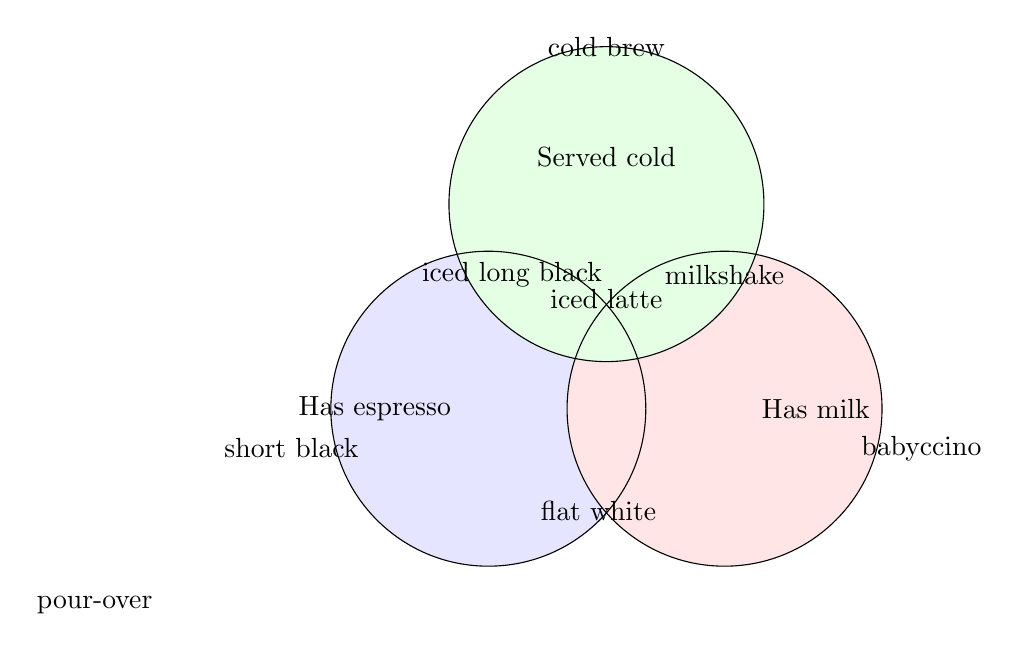
\begin{tikzpicture}[scale=1]
  % Parameters for Venn diagram
  \def\radius{2} % radius of circles
  \def\distanceEM{3} % distance between espresso and milk centers (horizontal)
  \def\distanceMC{3} % distance between milk and cold centers (used for equilateral triangle)
  % Circle positions forming an equilateral triangle
  \coordinate (E) at (0,0); % Has espresso
  \coordinate (M) at (\distanceEM,0); % Has milk
  \coordinate (C) at ({\distanceEM/2},{\distanceMC*sqrt(3)/2}); % Served cold

  % Draw circles with light fills for clarity
  \fill[blue!10] (E) circle (\radius);
  \fill[red!10] (M) circle (\radius);
  \fill[green!10] (C) circle (\radius);

  % Draw circle outlines and labels
  \draw (E) circle (\radius) node[left=10pt] {Has espresso};
  \draw (M) circle (\radius) node[right=10pt] {Has milk};
  \draw (C) circle (\radius) node[above=10pt] {Served cold};

  % Place drink names in appropriate Venn regions
  % Region definitions (approximate centers):
  % None of the sets (pour-over)
  \node at (-5,-2.5) {pour-over};
  % Only espresso (short black)
  \node at (-2.5,-0.5) {short black};
  % Only milk (babyccino)
  \node at (5.5,-0.5) {babyccino};
  % Only cold (cold brew)
  \node at (1.5,4.6) {cold brew};
  % Espresso + milk (not cold) (flat white)
  \node at (1.4,-1.3) {flat white};
  % Espresso + cold (not milk) (iced long black)
  \node at (0.3,1.7) {iced long black};
  % Milk + cold (not espresso) (milkshake)
  \node at (3,1.7) {milkshake};
  % All three (iced latte)
  \node at (1.5,1.4) {iced latte};
\end{tikzpicture}
\end{document}